
We now discuss the stability of PF and EnKF by calculating $\mathbb E[D_\varepsilon(\hat\pi_n(\mu_i), \hat\pi_n(\mu_j))], \ i \ne j$ as a function of time $n$ for initial conditions $\mu_i$ from~\eqref{eq-3ic--numerical-fs}, with the expectation taken by
averaging over $10$ observation realizations. For clarity, the above quantity is shown at every $4$-th assimilation step in figures~\ref{fig:plot-BPF--numerical-fs}--\ref{fig:plot-compare--numerical-fs}.

\subsection{Zero of the Sinkhorn algorithm}
% Sinkhorn zeros(reduce size, improve title)
\begin{figure}
\centering
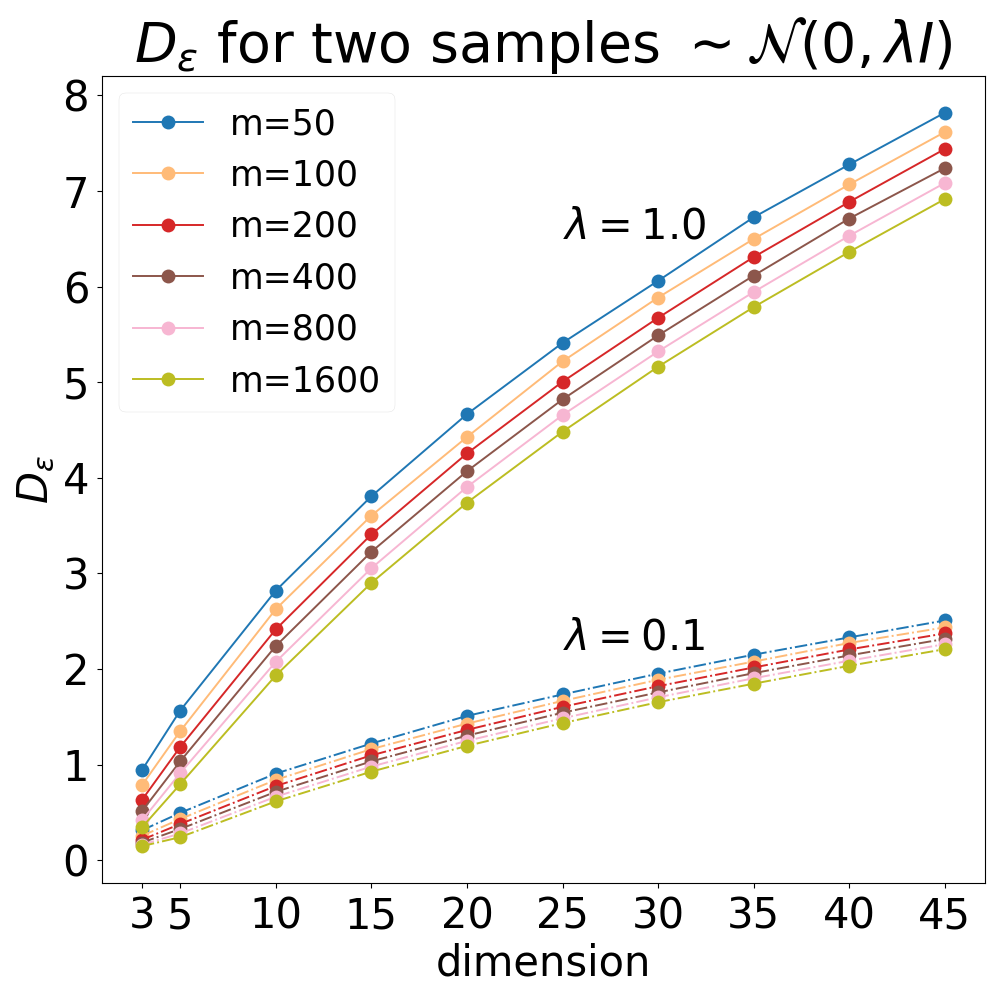
\includegraphics[width=0.8\columnwidth]{stability/plots/figures-EnKF-zeros_cov=0.1_cov=1.0.png}
\caption{Average $D_{\varepsilon}(\alpha_m^d, \beta_m^d)$ (over $20$ realizations) where $\alpha_m^d, \beta_m^d$ are two different sampling distributions with the same sample size $m$ for the same underlying $d$-dimensional Gaussian $\mathcal N(0_d, \lambda I_d)$}
\label{fig:plot-zeros--numerical-fs}
\end{figure}
In order to understand the convergence to $0$ of the above quantity [see~\eqref{eq-stablaw--numerical-fs}], we first discuss how close to zero $D_\varepsilon$ can approach numerically. In figure~\ref{fig:plot-zeros--numerical-fs} we see the average $D_\varepsilon(\alpha^d_m, \beta^d_m)$ where $\alpha_m^d=\frac{1}{m}\sum_{i=1}^m\delta_{x^{m,d}_i}$ and $\beta_m^d=\frac{1}{m}\sum_{i=1}^m\delta_{y^{m,d}_i}$, with $\{x^{m,d}_i\}$ and $\{y^{m,d}_i\}$ both samples from the same underlying $d$-dimensional Gaussian distribution $\mathcal N_d^\lambda:=\mathcal N(0_d, \lambda I_d)$. 
For `small' $\lambda$, we can expect $D_\varepsilon$ to behave in a similar fashion as if $\mathcal N_d^\lambda$ were supported on a compact set. With that in mind, we relate the numerical results shown in figure~\ref{fig:plot-zeros--numerical-fs} to the results~\ref{lem-prop--numerical-fs}--\ref{thm-zero--numerical-fs} in the appendix~\ref{sec-app--numerical-fs} by noting the following key points:

% By the phrase \textit{zero of the Sinkhorn algorithm} we mean the value of $D_\varepsilon$ obtained by using algorithm~\ref{algo-sink--numerical-fs} when the inputs are two different sampling distributions coming from the same underlying probability distribution.

\subsubsection{Drop with increase in sample size} Theorem~\ref{thm-zero--numerical-fs} explains the monotone drop in average $D_\varepsilon$ for a fixed dimension while increasing the sample size.

\subsubsection{Rise with increase in dimension} As the dimension increases, larger sample sizes are required to accurately estimate $\mathcal N_d^\lambda$. Consequently, $D_\varepsilon(\alpha_m^d, \beta_m^d)$ grows with $d$ for fixed $m$ since $\alpha_m^d, \beta_m^d$ become poorer estimators of $\mathcal N_d^\lambda$ as $d$ increases. 

 % PF 12 plots 
\begin{figure*}[!t]
\centering
\begin{subfigure}{0.3\textwidth}
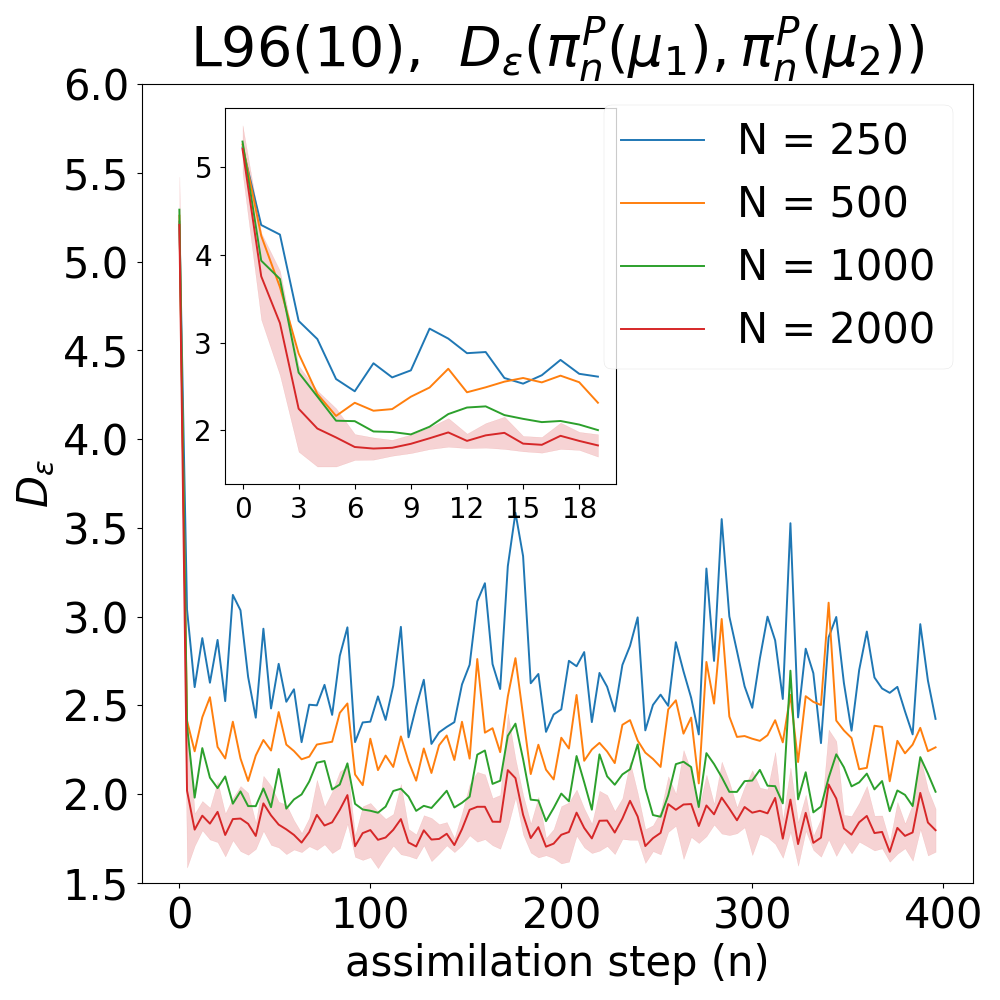
\includegraphics[width=\columnwidth]{stability/plots/figures-BPF-L96_10-1-dist_1_vs_2.png}
%\caption{dist 1 vs 2}
\end{subfigure}\hspace{0mm}%
\begin{subfigure}{0.3\textwidth}
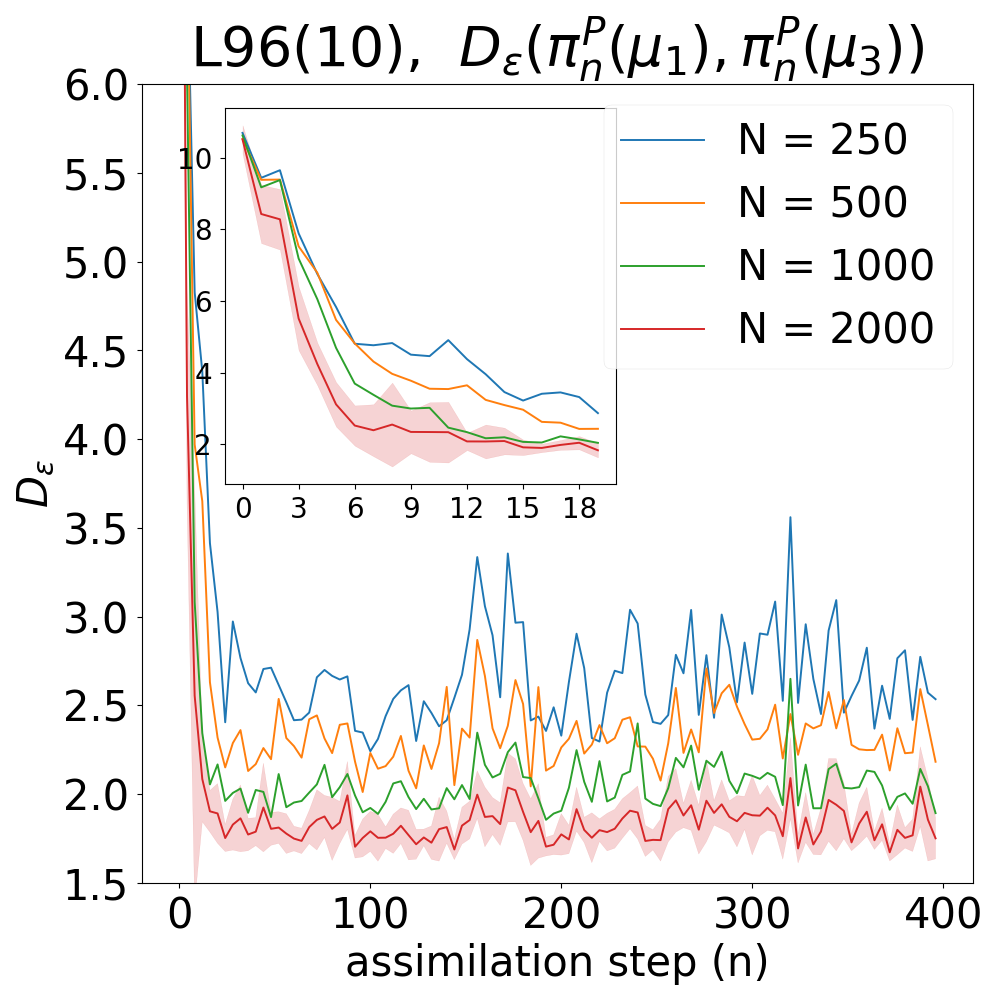
\includegraphics[width=\columnwidth]{stability/plots/figures-BPF-L96_10-1-dist_1_vs_3.png}
%\caption{dist 1 vs 3}
\end{subfigure}\hspace{0mm}%
\begin{subfigure}{0.3\textwidth}
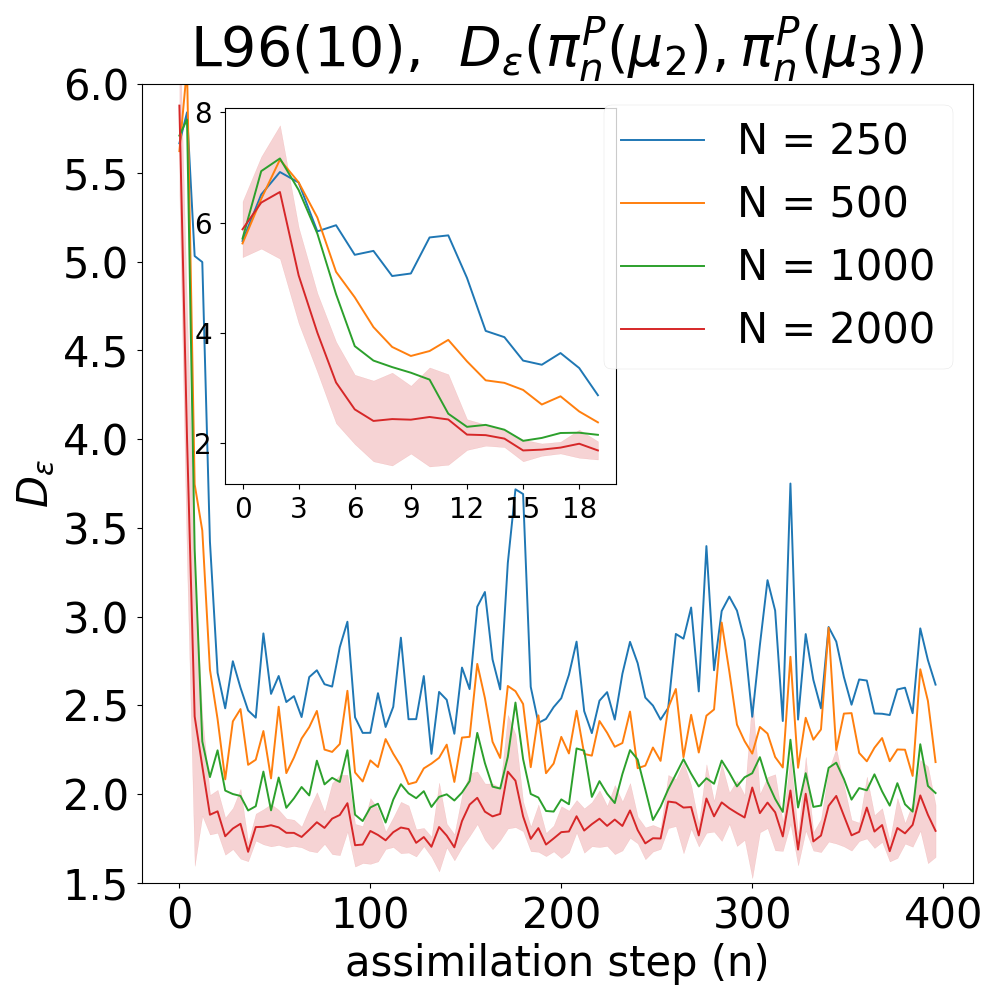
\includegraphics[width=\columnwidth]{stability/plots/figures-BPF-L96_10-1-dist_2_vs_3.png}
%\caption{dist 2 vs 3}
\end{subfigure}\hspace{0mm}%

\begin{subfigure}{0.3\textwidth}
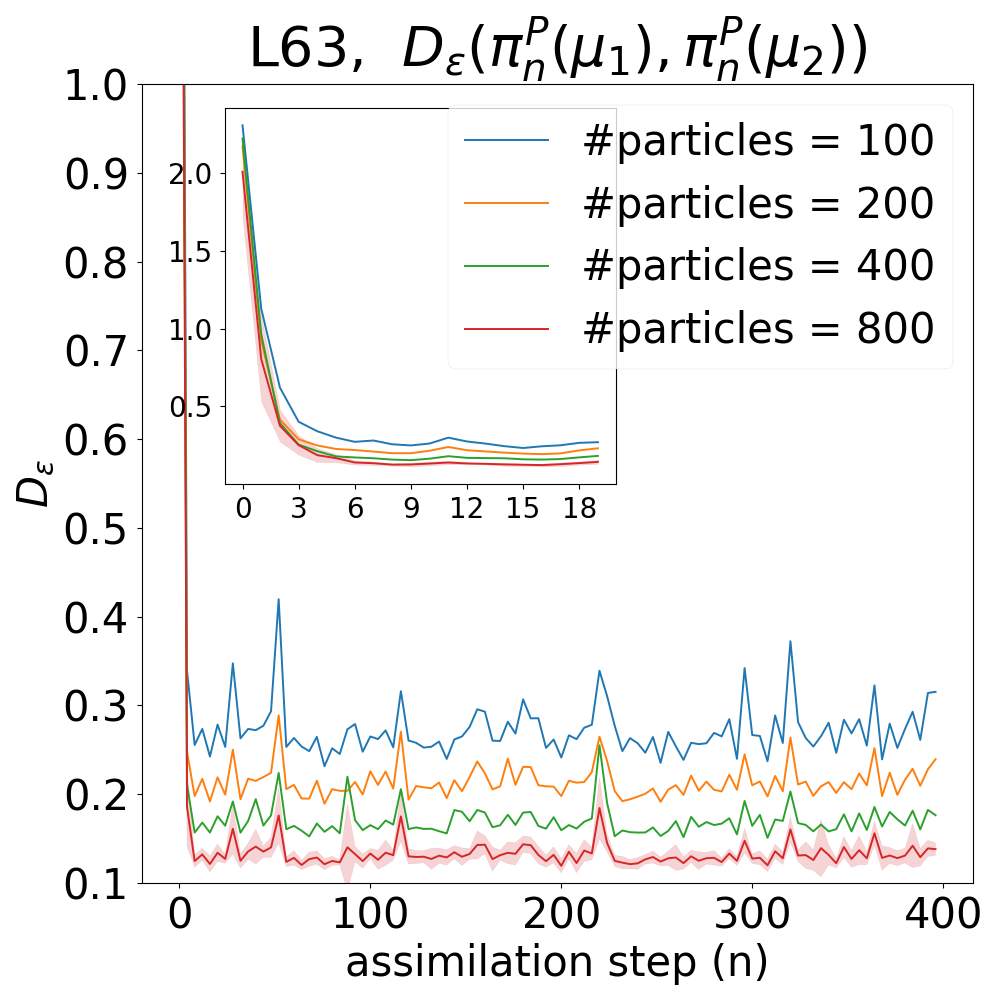
\includegraphics[width=\columnwidth]{stability/plots/figures-BPF-L63-1-dist_1_vs_2.png}
%\caption{dist 1 vs 2}
\end{subfigure}\hspace{0mm}%
\begin{subfigure}{0.3\textwidth}
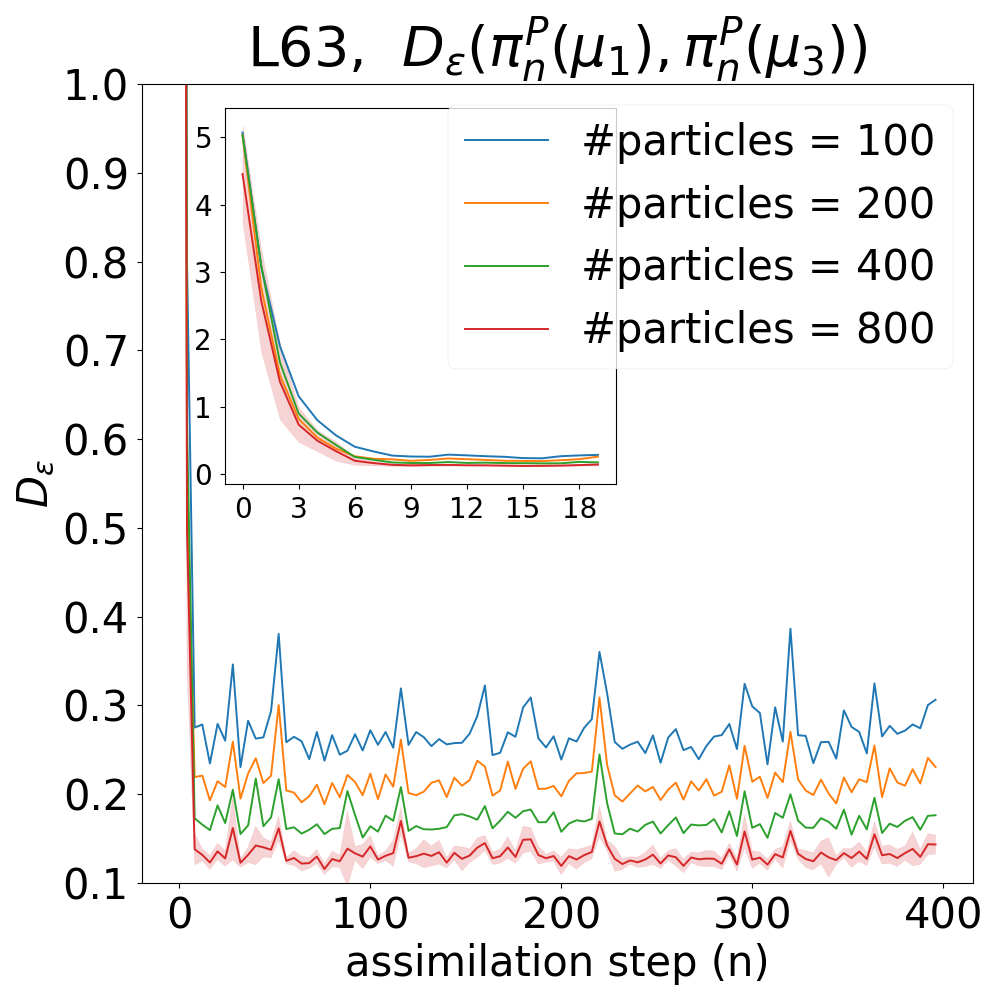
\includegraphics[width=\columnwidth]{stability/plots/figures-BPF-L63-1-dist_1_vs_3.png}
%\caption{dist 1 vs 3}
\end{subfigure}\hspace{0mm}%
\begin{subfigure}{0.3\textwidth}
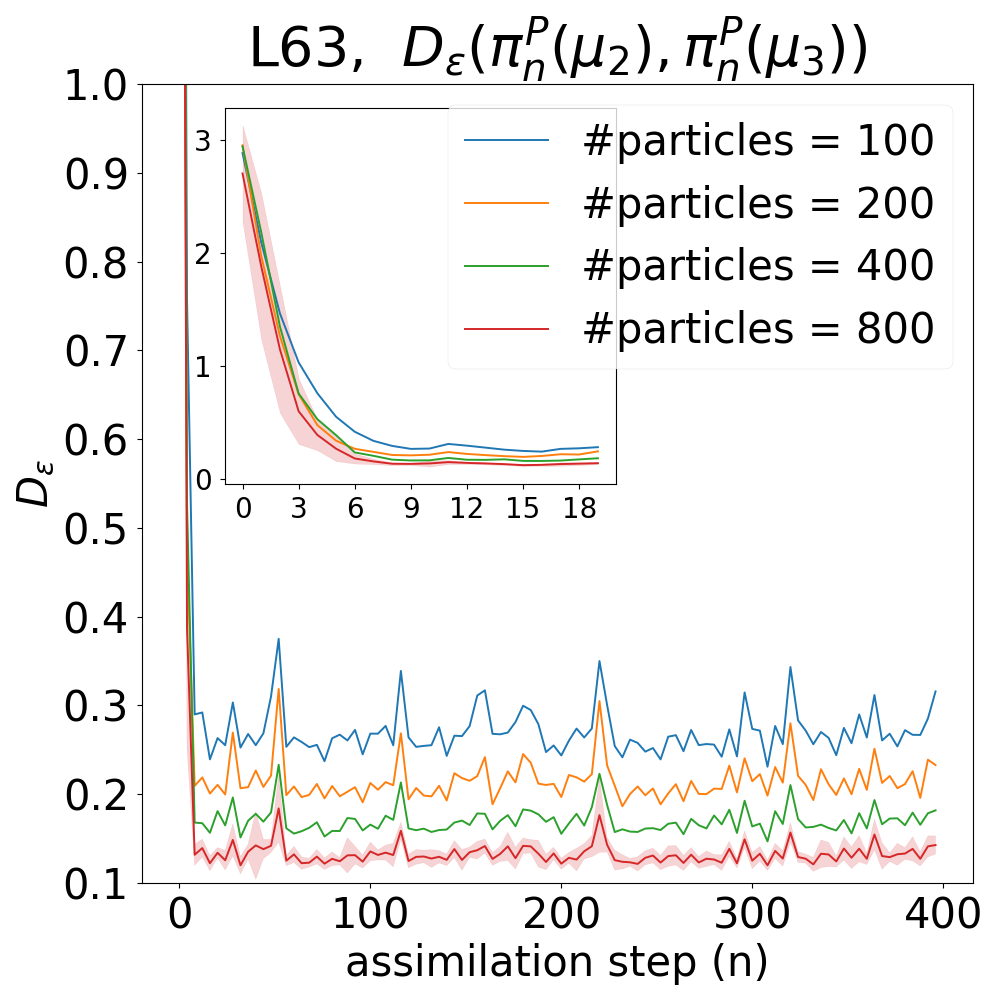
\includegraphics[width=\columnwidth]{stability/plots/figures-BPF-L63-1-dist_2_vs_3.png}
%\caption{dist 2 vs 3}
\end{subfigure}\hspace{0mm}
\caption{$D_\varepsilon$ (averaged over $10$ observation realizations) for BPF for $10$-dimensional $L96$ (row 1) and $L63$ (row 2) systems with observation covariance $\sigma^2=0.1$, for pairs of initial distributions in~\eqref{eq-3ic--numerical-fs}, with varying sample size. The line for $N = 2000$ has a band showing one standard deviation. The inset shows the drop in average $D_\varepsilon$ during the first few assimilation steps.}
\label{fig:plot-BPF--numerical-fs}
\end{figure*}

\subsubsection{Drop with decrease in covariance} Decreasing the covariance $\lambda$ has the opposite effect since, for fixed dimension $d$ and sample size $m$, smaller covariance leads to a better estimation of the underlying distribution, i.e., $\alpha_m^d, \beta_m^d$ become better estimators of $\mathcal N_d^\lambda$ as $\lambda$ decreases.

\subsubsection{Support of our distributions} Since the true trajectories for both systems (L63, L96) lie on bounded attractors, we can assume that true filtering distributions are supported on a compact set. Consequently, in the filtering experiments shown later, the zero of the Sinkhorn algorithm shows qualitatively similar behavior (e.g., in figure~\ref{fig:plot-BPF--numerical-fs}) with respect to dimension as seen in figure~\ref{fig:plot-zeros--numerical-fs}.

\subsection{Particle Filter}
Here we use the notation $\pi^{P, N}_n$ for $\hat\pi_n$ obtained by alogithm~\ref{algo-bpf--numerical-fs} with $N$ particles (omitting $N$ for brevity when value of $N$ is clear from context). Figure~\ref{fig:plot-BPF--numerical-fs} shows $\mathbb E[D_\varepsilon(\hat\pi_n(\mu_i), \hat\pi_n(\mu_j))], \ i \ne j$ as a function of $n$. We note some important conclusions.
\subsubsection{BPF quickly forgets the initial distribution} From the insets in figure~\ref{fig:plot-BPF--numerical-fs} we can see that for every pair $(\mu_i, \mu_j)$ of initial distributions, $\mathbb E\left[D_\varepsilon(\pi^P_n(\mu_i), \pi^P_n(\mu_j))\right]$ stabilizes in the first few assimilation steps. In fact, this behavior is consistent with exponential stability of particle filters \cite{chigansky2009intrinsic}.
\subsubsection{Dependence on the number of particles} 
$\mathbb E\left[D_\varepsilon(\pi^{P, N}_n(\mu_i), \pi^{P, N}_n(\mu_j))\right]$ for a fixed $n$ decreases monotonically with increasing $N$ for both L63 and L96 and for both observation covariances for all pairs $i\neq j$.
%$\pi^{P,N}_n$ weak$^*$ converges to the true filtering distribution $\pi_n$ as $N\to\infty$ \cite{van2008hidden}. This fact along with theorem \ref{thm-zero--numerical-fs} is enough for explaining the drop in $D_\varepsilon$ in figure~\ref{fig:plot-BPF--numerical-fs} for fixed $n$ as we increase $N$.
\subsubsection{Stability}
Suppose the best possible filtering distribution that can be computed by the particle filter is $\pi^{P,*}_n=\lim_{N\to\infty}\pi^{P,N}_n$. Figure~\ref{fig:plot-BPF--numerical-fs} is consistent with the condition
\begin{align*}
    \lim_{n\to\infty}\liminf_{N\to\infty}\mathbb E[D_\varepsilon(\pi^{P,N}_n(\mu_i), \pi^{P,N}_n(\mu_j))]=0\;\forall\; i\neq j
\end{align*}
since fixing $n$ and increasing $N$ results in a steady drop in $D_\varepsilon$ averaged over observation realizations. By theorem \ref{thm-stable--numerical-fs} this condition is sufficient for concluding
\begin{align*}
    \lim_{n\to\infty}\mathbb E[D_\varepsilon(\pi^{P,*}_n(\mu_i), \pi^{P,*}_n(\mu_j))]=0\;\forall\; i\neq j
\end{align*}
\subsubsection{Dependence on observation covariance} All plots in figure~\ref{fig:plot-BPF--numerical-fs} correspond to observation covariance $\sigma^2=0.1$. The other case $\sigma^2=1.0$ mentioned in \ref{ssec-models--numerical-fs} results in plots that are qualitatively similar to the ones in figure~\ref{fig:plot-BPF--numerical-fs} and we omit those plots here. In our experiments, stability of particle filter was not seen to be affected by observation covariance. 

\subsection{EnKF}
% Enkf 3 plot, 1 is left:
\begin{figure*}[!t]
\centering
\begin{subfigure}{.3\textwidth}
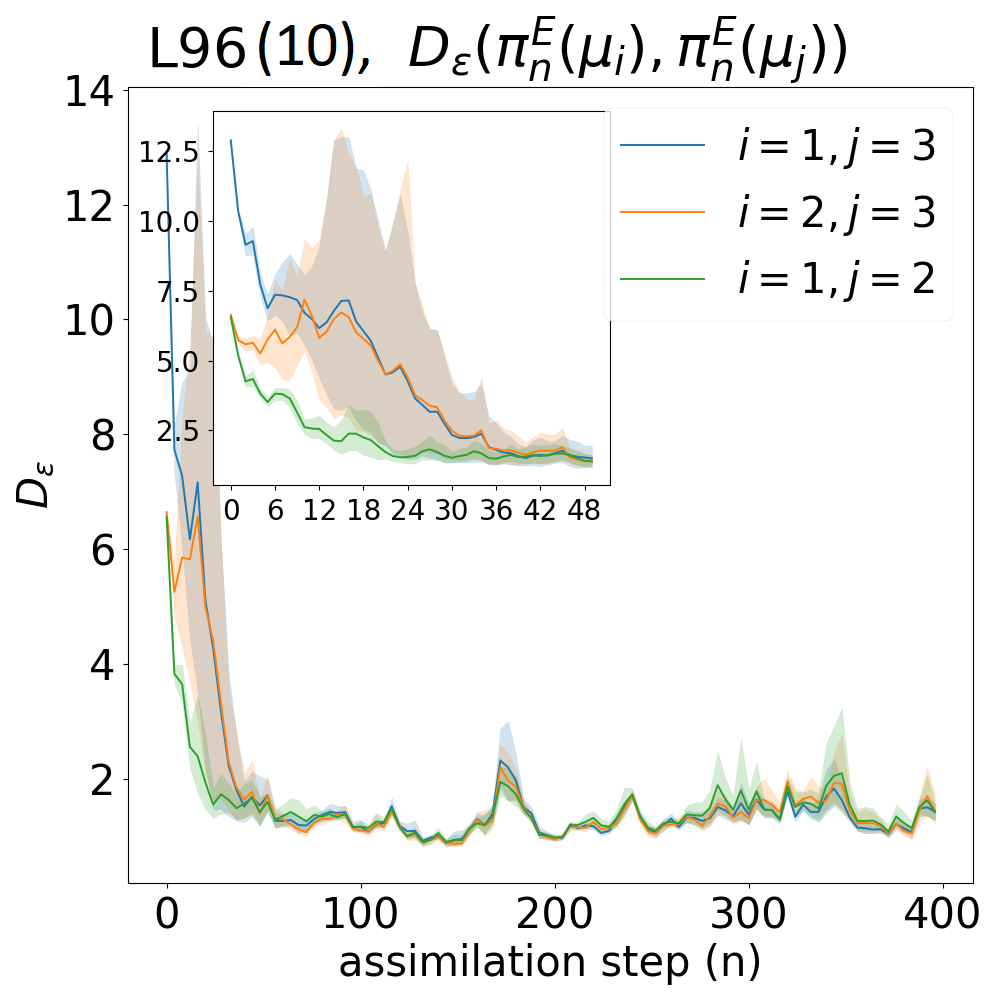
\includegraphics[width=\columnwidth]{stability/plots/figures-EnKF-stable_50_L96_10dim.png}%
%\caption{N=50 with localization}%
%\label{sub@fig:plot-enkf50--numerical-fs}%
\end{subfigure}\hspace{0mm}% 
\begin{subfigure}{.3\textwidth}
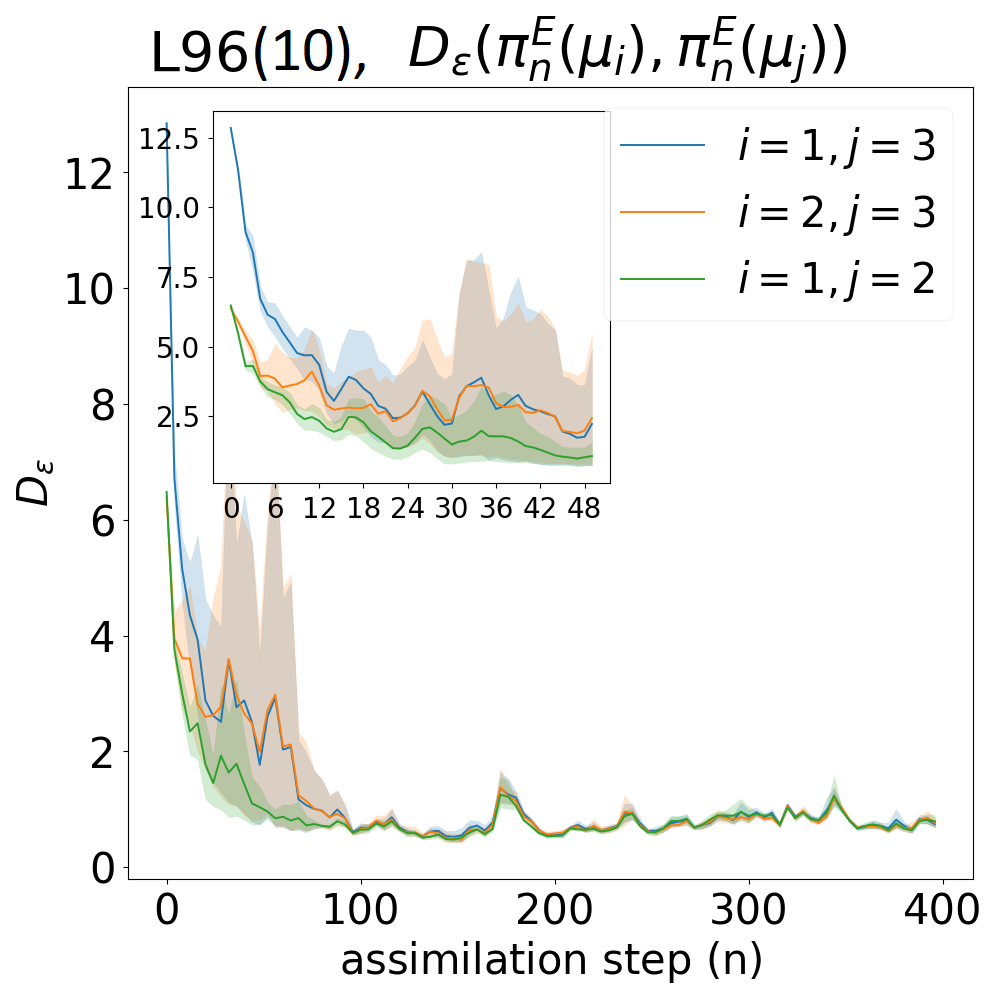
\includegraphics[width=\columnwidth]{stability/plots/figures-EnKF-stable_200_L96_10dim.png}%
%\caption{N=200 without localization}%
%\label{sub@fig:plot-enkf200--numerical-fs}%
\end{subfigure}\hspace{0mm}%
\begin{subfigure}{.3\textwidth}
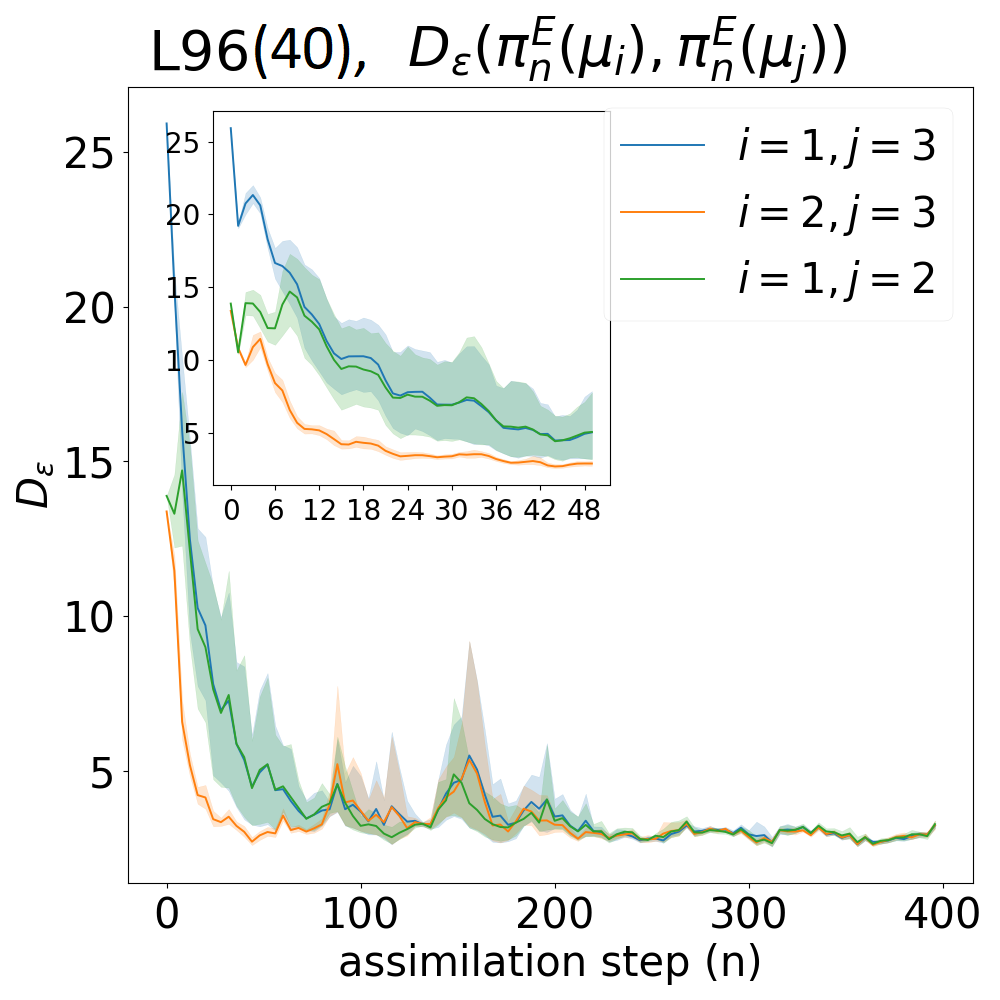
\includegraphics[width=\columnwidth]{stability/plots/figures-EnKF-stable_50_loc_L96_40dim.png}%
%\caption{$D_\varepsilon$ for $\mu_{i}$ with N=50,200}%
%\label{sub@fig:plot-enkfL96-40--numerical-fs}%
\end{subfigure}%
\caption{$D_\varepsilon$ (averaged over $10$ observation realizations, with one standard deviation confidence band) for EnKF for $10$-dimensional L96 with $N=50$ with localization (left), $N=200$ without localization (middle) for observation covariance $\sigma^2=0.1$, and for $40$-dimensional L96 with $N=50$ with localization (right) with observation covariance $\sigma^2=1.0$ for pairs of initial distributions in \ref{eq-3ic--numerical-fs}. The inset shows the drop in $D_\varepsilon$ for the first 50 assimilation steps.}
\label{fig:plot-enkfL96-10--numerical-fs}
\end{figure*}
Here we use the notation $\pi^{E,N}_n$ for $\hat\pi_n$ obtained by alogithm~\ref{algo-enkf--numerical-fs} with ensemble size $N$. We might omit $N$ for brevity.
\subsubsection{Drop in $D_\varepsilon$ over time}
From figure~\ref{fig:plot-enkfL96-10--numerical-fs}, we see that for every pair $(\mu_i, \mu_j)$ of initial distributions $D_\varepsilon(\pi^E_n(\mu_i), \pi^E_n(\mu_j))$ decreases with time rapidly within the first $50$ assimilation steps and beyond $100$ assimilation steps, the observation average of $D_\varepsilon$ for filters with different pairs initial distributions are similar and have very little variance.
\subsubsection{Variation with respect to observation realization} We see that the variation of $D_\varepsilon$ for different observation realizations (shown by the shaded bands in left two panels in figure~\ref{fig:plot-enkfL96-10--numerical-fs} and in top row in figure~\ref{fig:plot-BPF--numerical-fs}) is larger for the case of EnKF when compared to the particle filter for initial times (e.g. $n < 100$ for the 10-dimensional L96 model). On the other hand, for larger times (approx.~$n > 100$), the variation for EnKF is significantly smaller than the particle filter.
% \subsubsection{}
% For $10$-dimensional L96 system, we see that the $D_\varepsilon$ between the filer with localization and without localization for the same initial distribution are different but stable.  
\subsubsection{Effect of localization}
EnKF with small ensemble size needs localization which, however, is an ad-hoc procedure to prevent filter divergence and may not approximate the true filter. Figure~\ref{fig:plot-enkfL96-10--numerical-fs} for $10$-dimensional L96 (left panel) and for $40$-dimensional L96 (right panel) shows that for $N=50$ with localization length 4, the EnKF is stable, whereas the middle panel shows the stability (with the same configuration as the left panel) for $10$-dimensional L96 without localization, but with larger ensemble size $N=200$. This indicates that that localization does not affect EnKF's stability properties.

% L96-40 dimensions plot
% \begin{figure}
% \centering
% 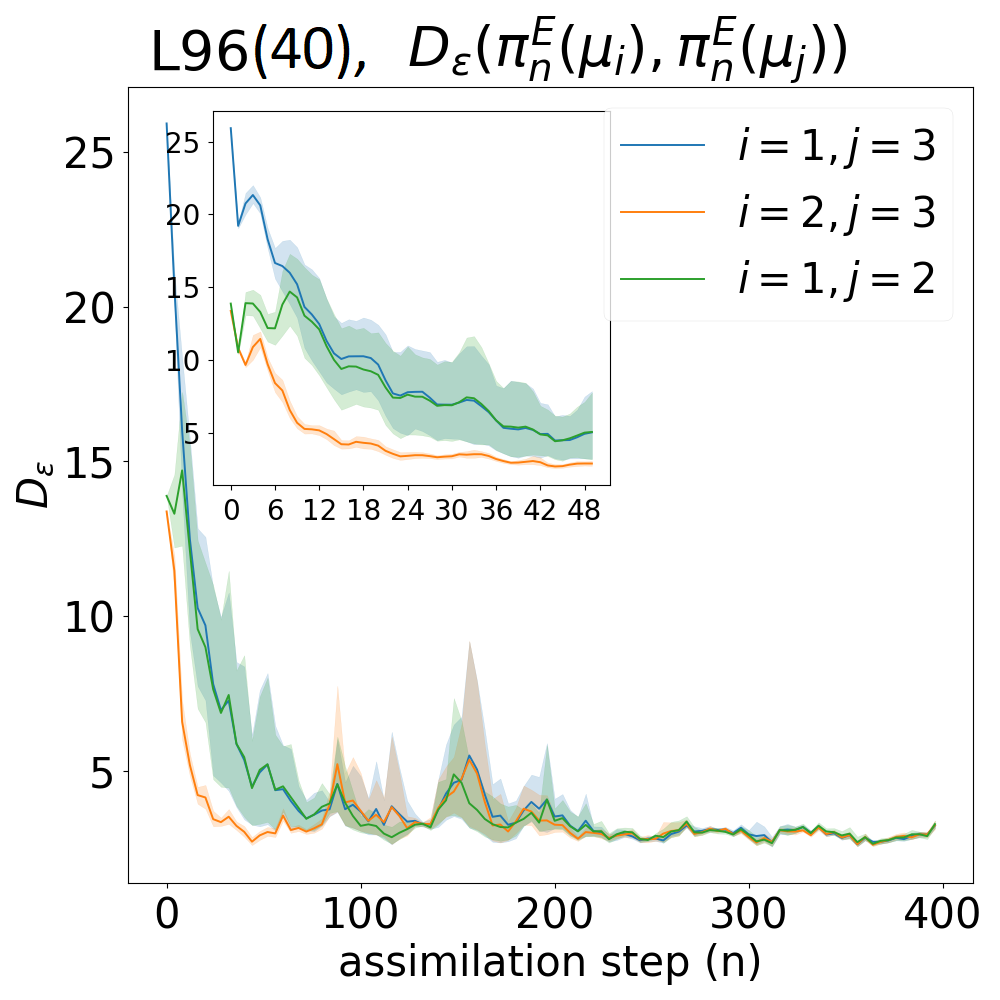
\includegraphics[width=0.8\columnwidth]{stability/plots/figures-EnKF-stable_50_loc_L96_40dim.png}
% \caption{$D_\varepsilon$ for $40$-dimensional L96 model for N=50 with localization length=4.}
% \label{fig:plot-enkfL96-40--numerical-fs}
% \end{figure}

\subsection{BPF vs EnKF}
\begin{figure}
\centering
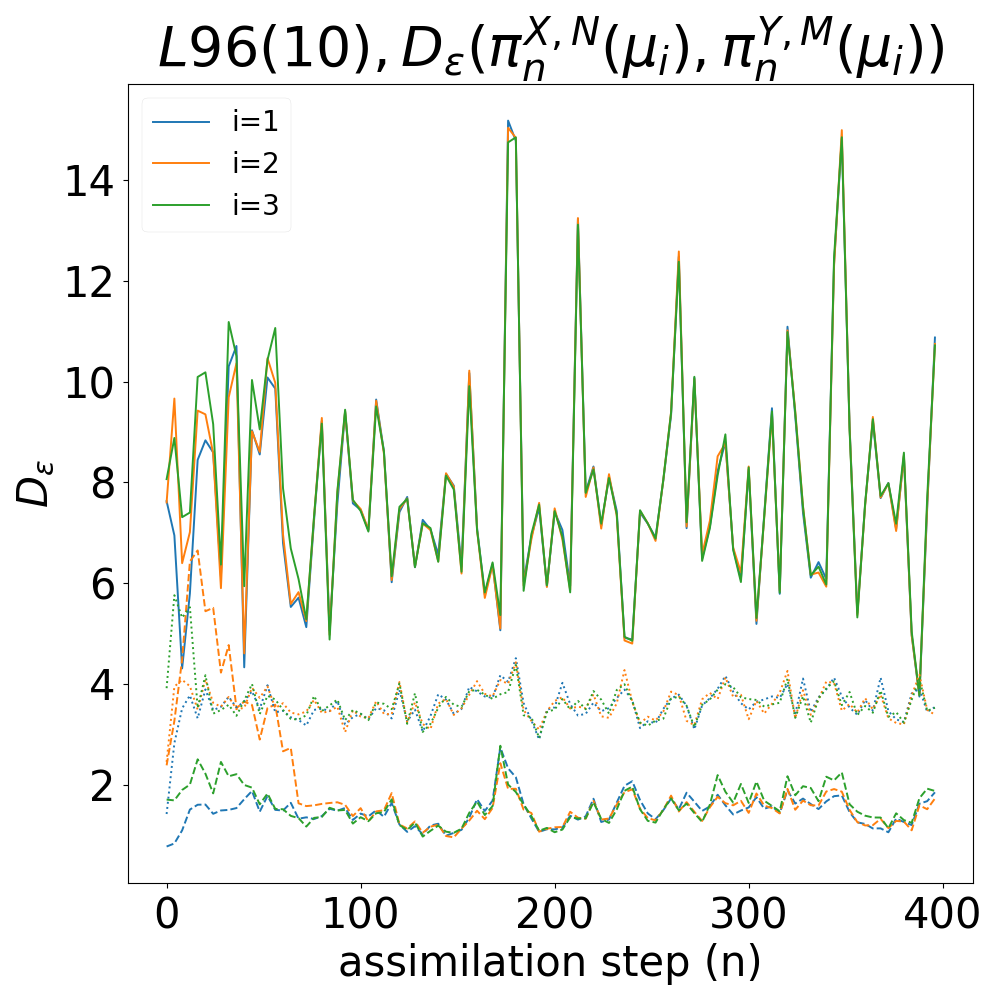
\includegraphics[width=0.8\columnwidth]{stability/plots/figures-BPF-L96_10-EnKF-distance between different filters.png}
\caption{Comparison between filters for $10$-dimensional L96 and $\sigma^2=1.0$. The solid lines on the top show average $D_\varepsilon$ between EnKF without localization with $N = 200$ and BPF with $M = 2000$. The dotted lines in the middle show average  $D_\varepsilon$ between  BPF with $N = 250$ and BPF with $M = 2000$. The dashed lines at the bottom show average  $D_\varepsilon$ between EnKF without localization with $N = 200$ and EnKF with localization with $M = 50$. In each case, different colors are for different initial conditions from~\eqref{eq-3ic--numerical-fs}.} 
\label{fig:plot-compare--numerical-fs}
\end{figure}
We now compare the BPF and EnKF for the case of $10$-dimensional L96 with $\sigma^2=1.0$ with the same true trajectory and observation realizations. This is shown in figure~\ref{fig:plot-compare--numerical-fs}. {In the following discussion we assume BPF with 2000 particles to be a decent approximation for the true filter and refer to them interchangably.} We note a few important points.
\subsubsection{Poor approximation of the true filter by EnKF} The three lines towards the top show the distance between EnKF and BPF, for three different initial conditions. We see that EnKF produces distributions that are significantly different from the true filter, for all the initial distributions. But recall that for this setup, the EnKF is stable (as is the BPF too), i.e., the distance between EnKF with different initial conditions is smaller (as seen in figures~\ref{fig:plot-BPF--numerical-fs}-\ref{fig:plot-enkfL96-10--numerical-fs}) than the distance between the BPF and EnKF
\subsubsection{BPF is closer to the true filter than is EnKF} The three lines in the middle show the distance between BPF with $N=250$ and $N=2000$ (putatively true filter). We see that in comparison with EnKF with $N=200$ particles, BPF with similar ensemble size (250 particles) is much closer to the true filter.
\subsubsection{EnKF with different ensemble size are very similar} The bottom three lines in figure~\ref{fig:plot-compare--numerical-fs} show $D_\varepsilon$ between EnKF with different ensemble size, which shows that the EnKF is quite stable with respect to changes in the ensemble size, even though it is not very close to the true filter -- thus EnKF is stable but biased, whereas BPF is stable and unbiased. A more detailed study of the reasons for this behaviour will be taken up in the future.

% %trial and all error : this is to be removed.
% \begin{figure*}
% \centering
% %\begin{tabular}{ccc}
% \subcaptionbox{caption\label{1--numerical-fs}}{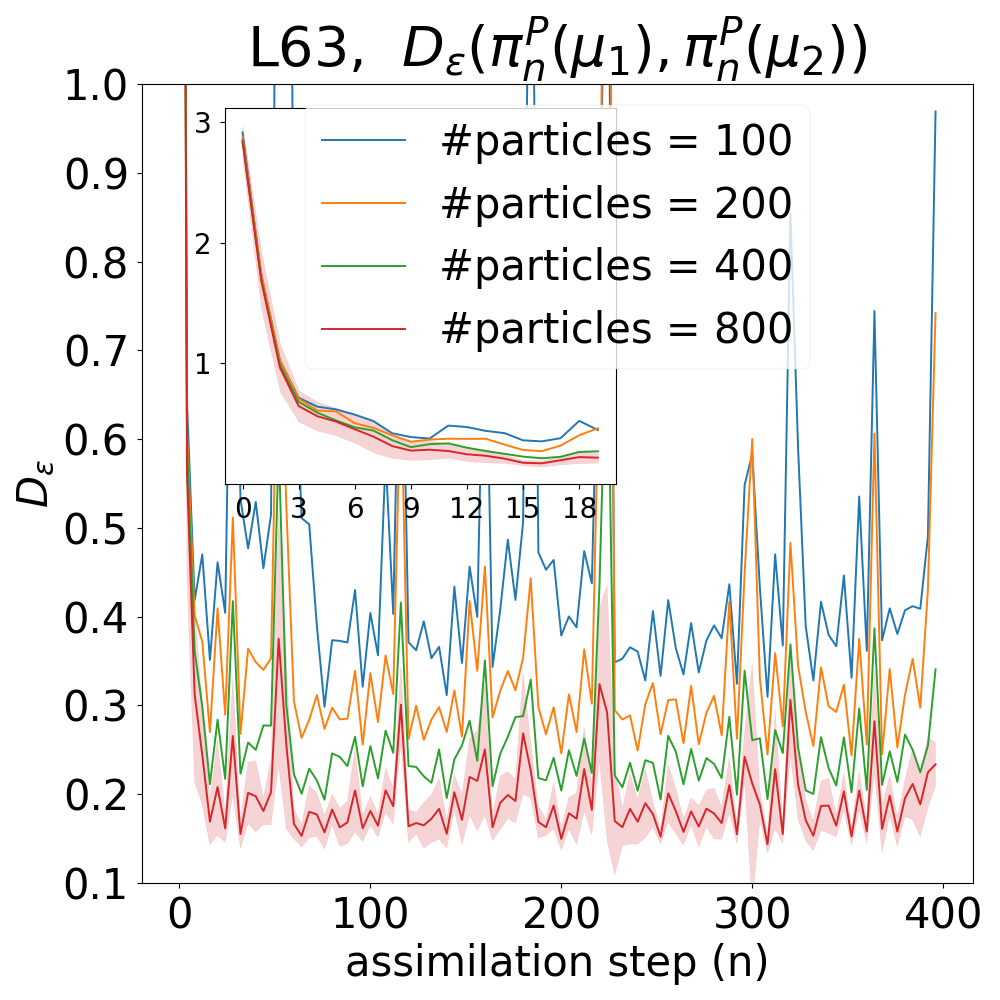
\includegraphics[width=0.28\textwidth]{stability/plots/figures-BPF-L63-0-dist_1_vs_2.png}}\hspace{0mm}
% \subcaptionbox{caption\label{2--numerical-fs}}{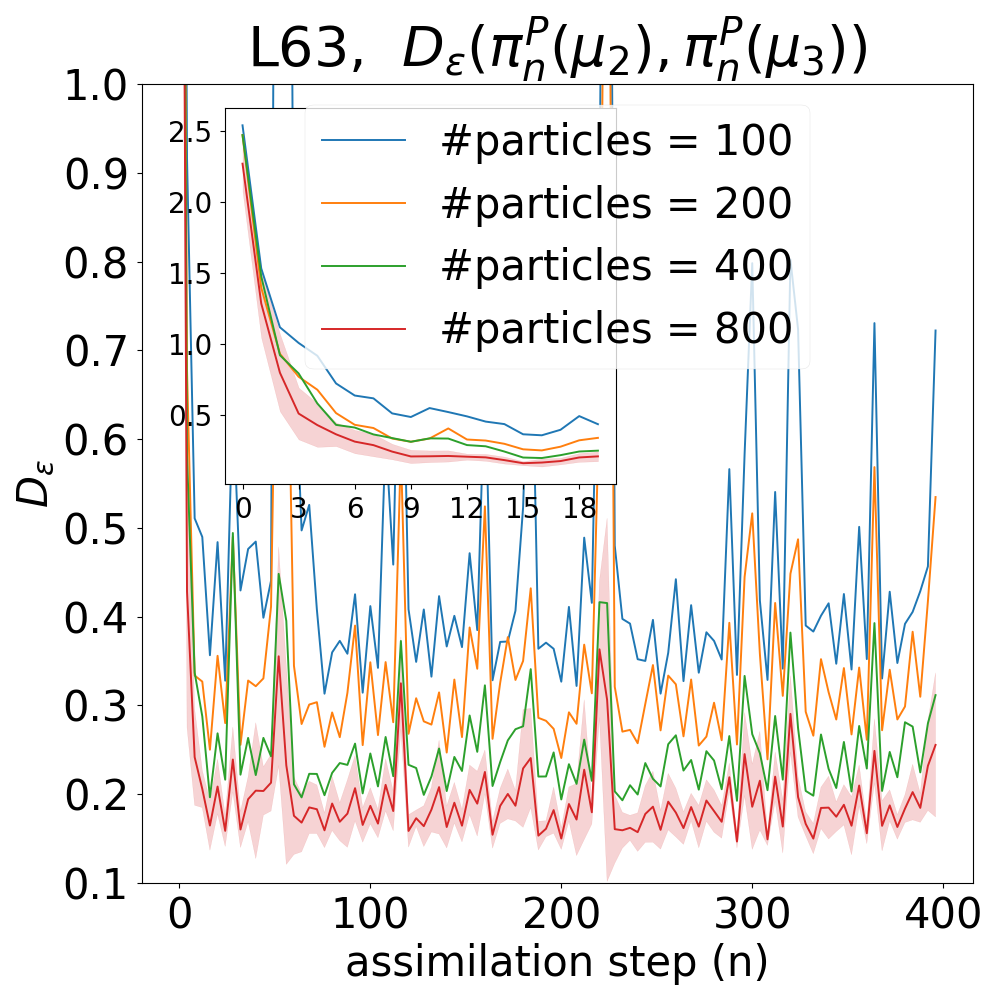
\includegraphics[width =0.28\textwidth]{stability/plots/figures-BPF-L63-0-dist_2_vs_3.png}}\hspace{0mm}
% \subcaptionbox{caption\label{2--numerical-fs}}{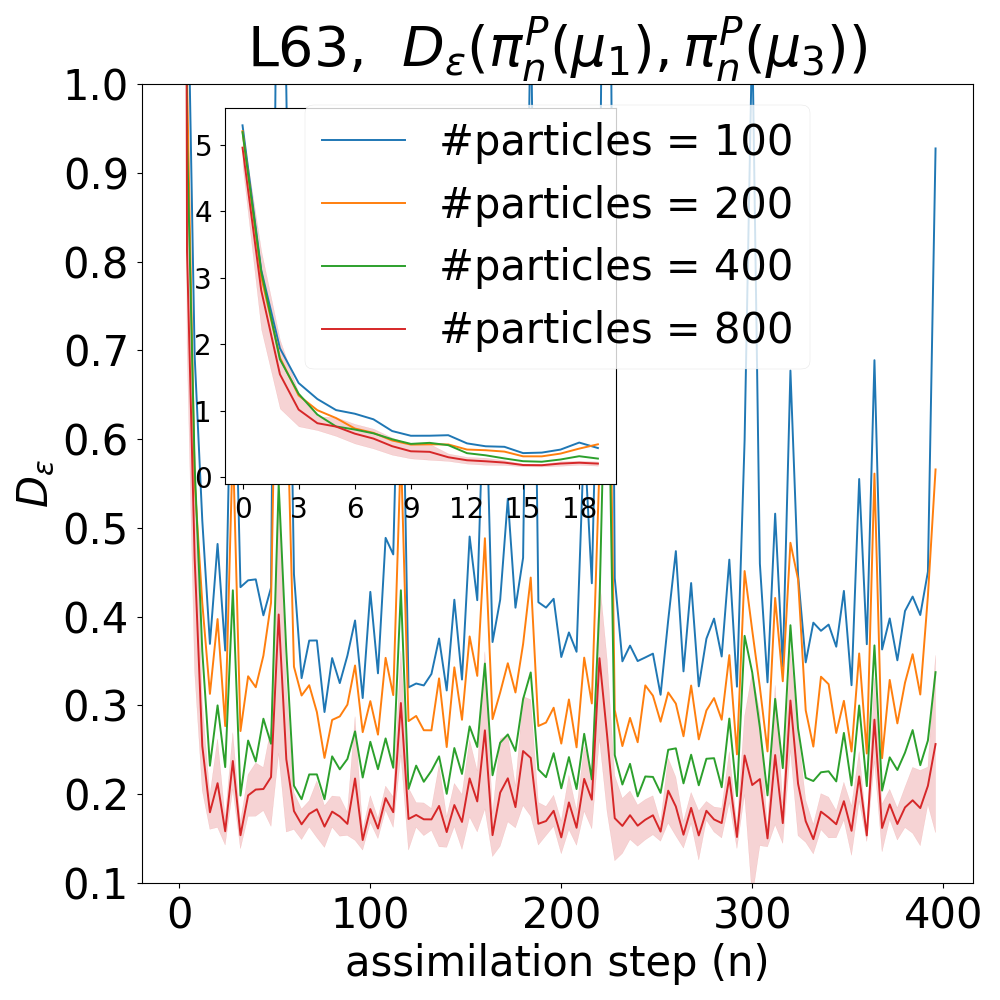
\includegraphics[width = 0.28\textwidth]{stability/plots/figures-BPF-L63-0-dist_1_vs_3.png}}\hspace{0mm}//%
% \subcaptionbox{caption\label{1--numerical-fs}}{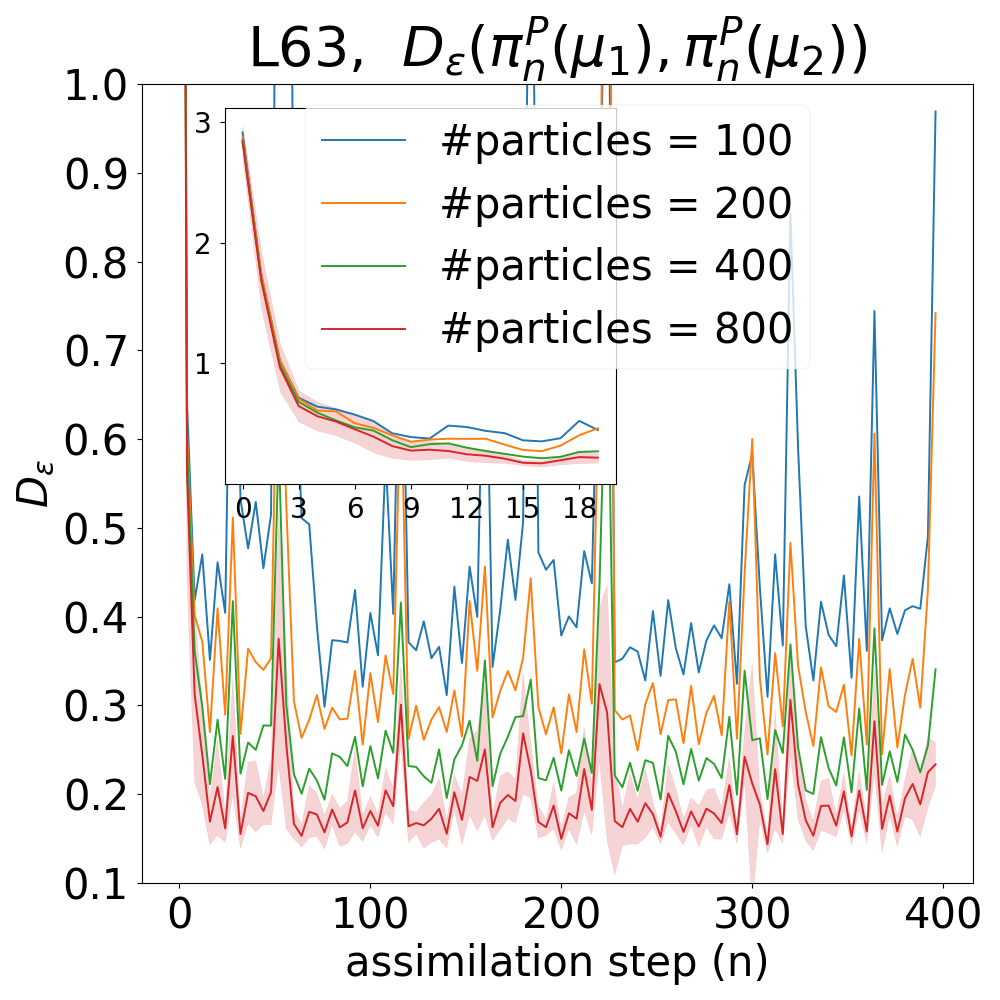
\includegraphics[width=0.28\textwidth]{stability/plots/figures-BPF-L63-0-dist_1_vs_2.png}}\hspace{0mm}
% \subcaptionbox{caption\label{2--numerical-fs}}{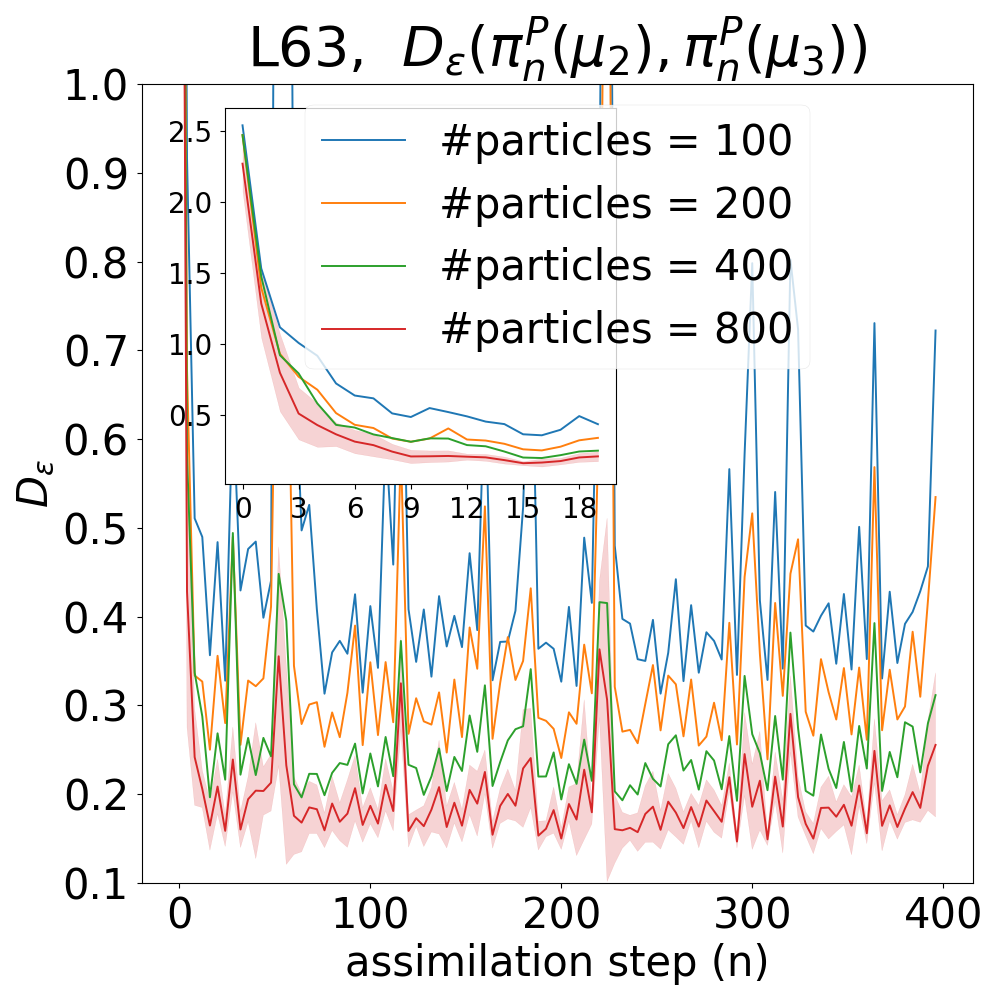
\includegraphics[width =0.28\textwidth]{stability/plots/figures-BPF-L63-0-dist_2_vs_3.png}}\hspace{0mm}
% \subcaptionbox{caption\label{2--numerical-fs}}{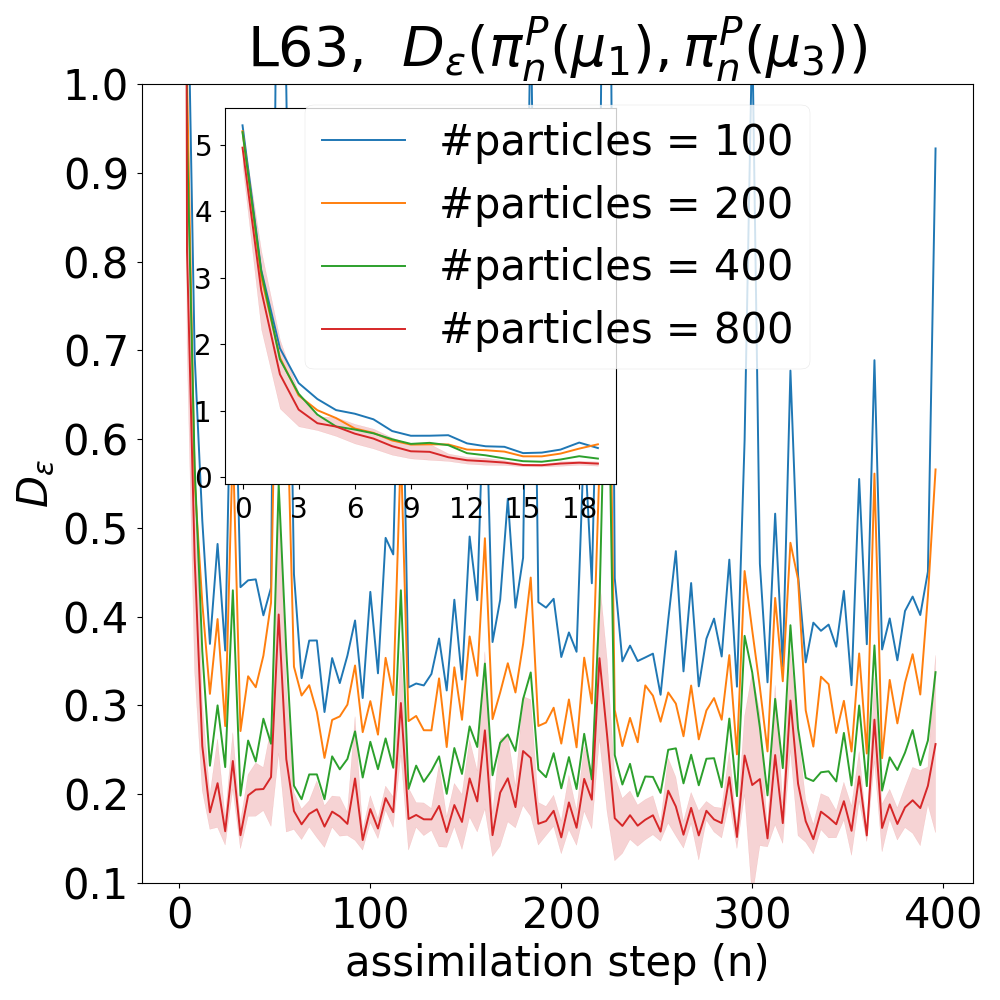
\includegraphics[width = 0.28\textwidth]{stability/plots/figures-BPF-L63-0-dist_1_vs_3.png}}\hspace{0mm}//
% %\end{tabular}
% \caption{caption}
% \label{fig2--numerical-fs}
% \end{figure*}

% \begin{figure*}[p]
% \begin{tabular}{c|c|c|c}

% {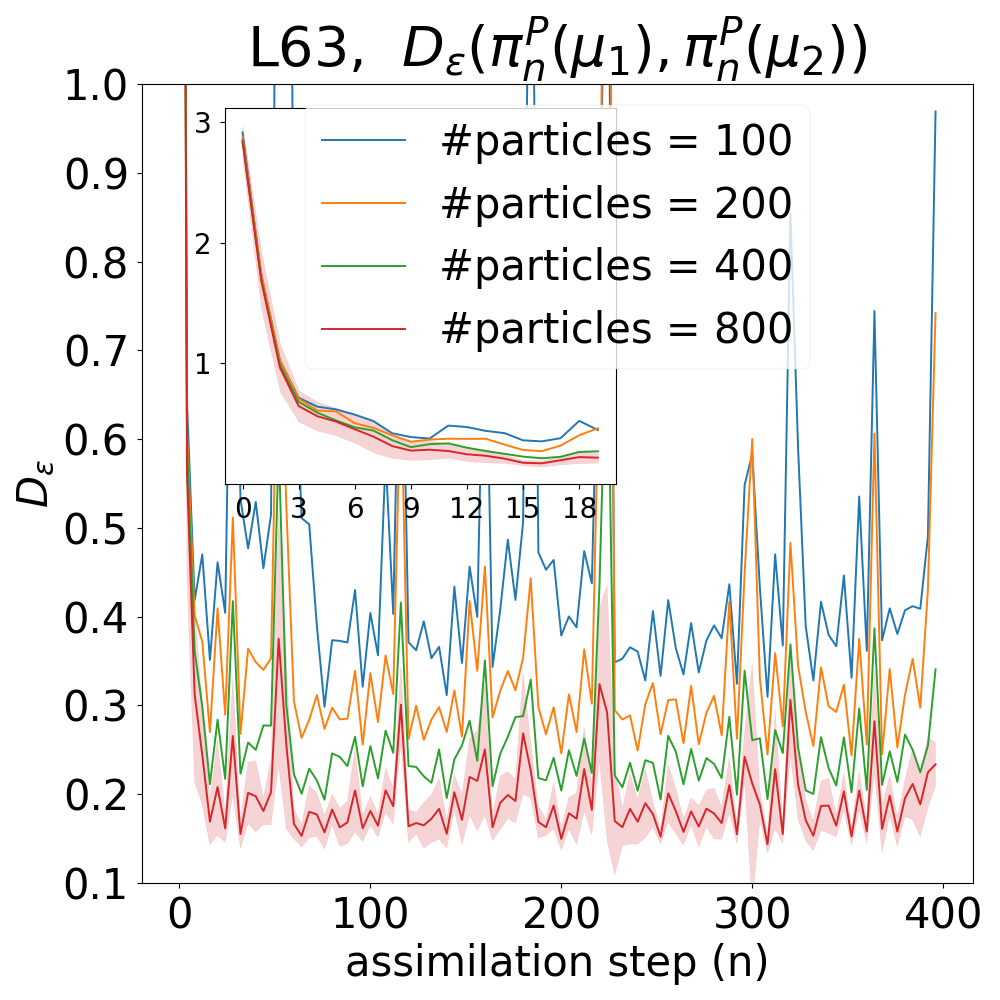
\includegraphics[width=0.2\textwidth]{stability/plots/figures-BPF-L63-0-dist_1_vs_2.png}} &
% {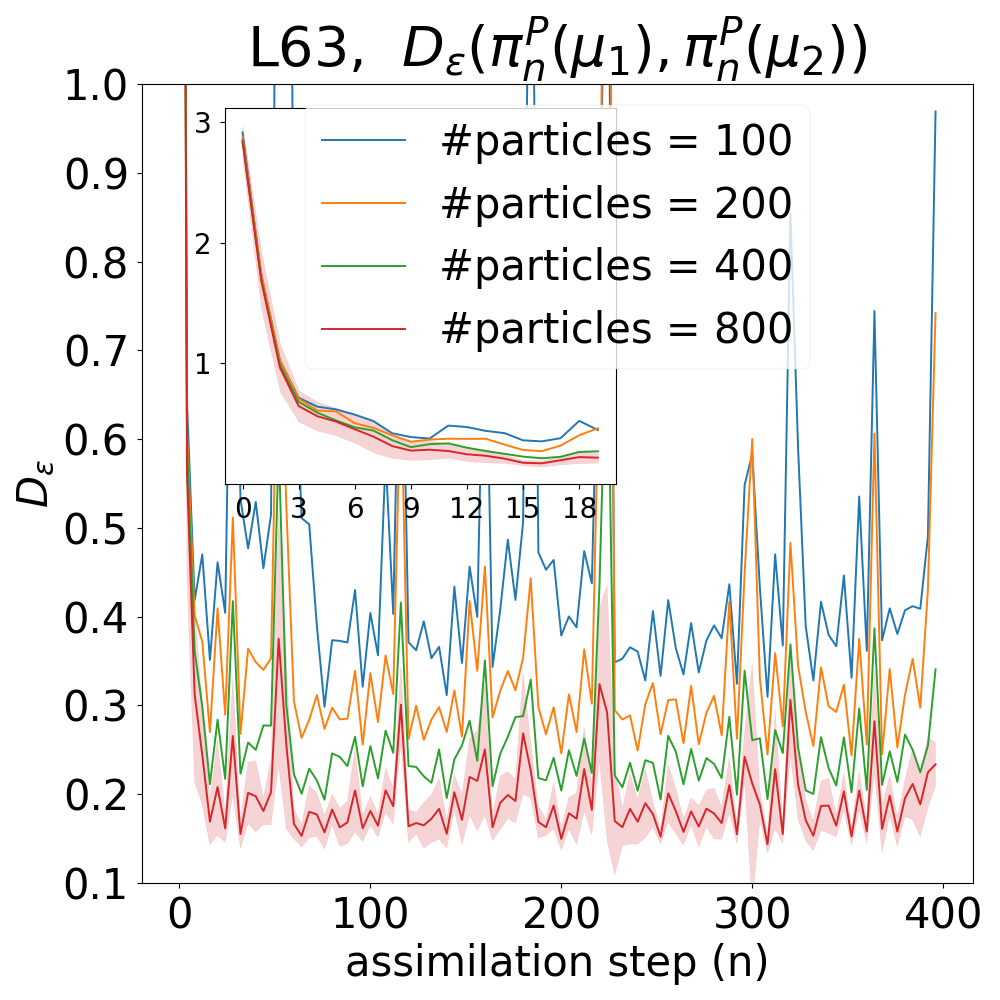
\includegraphics[width=0.2\textwidth]{stability/plots/figures-BPF-L63-0-dist_1_vs_2.png}} &
% {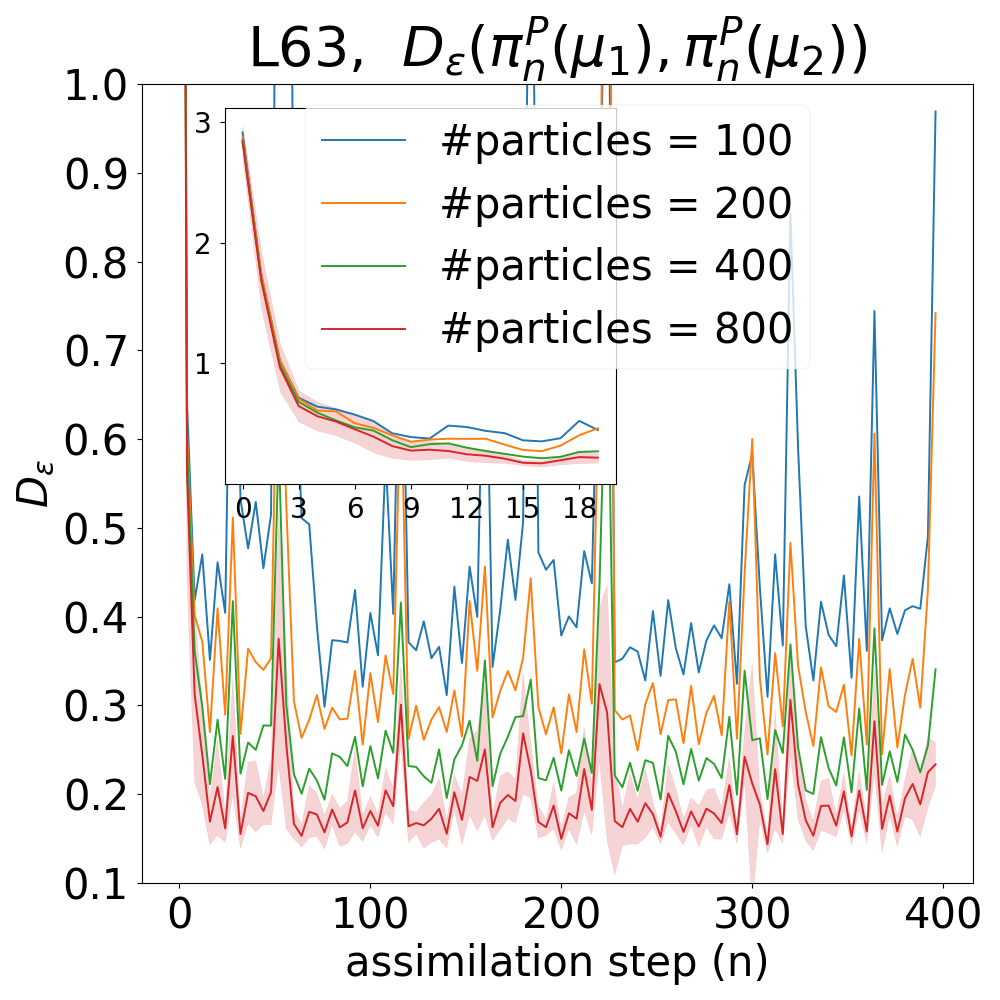
\includegraphics[width=0.2\textwidth]{stability/plots/figures-BPF-L63-0-dist_1_vs_2.png}} \\

% {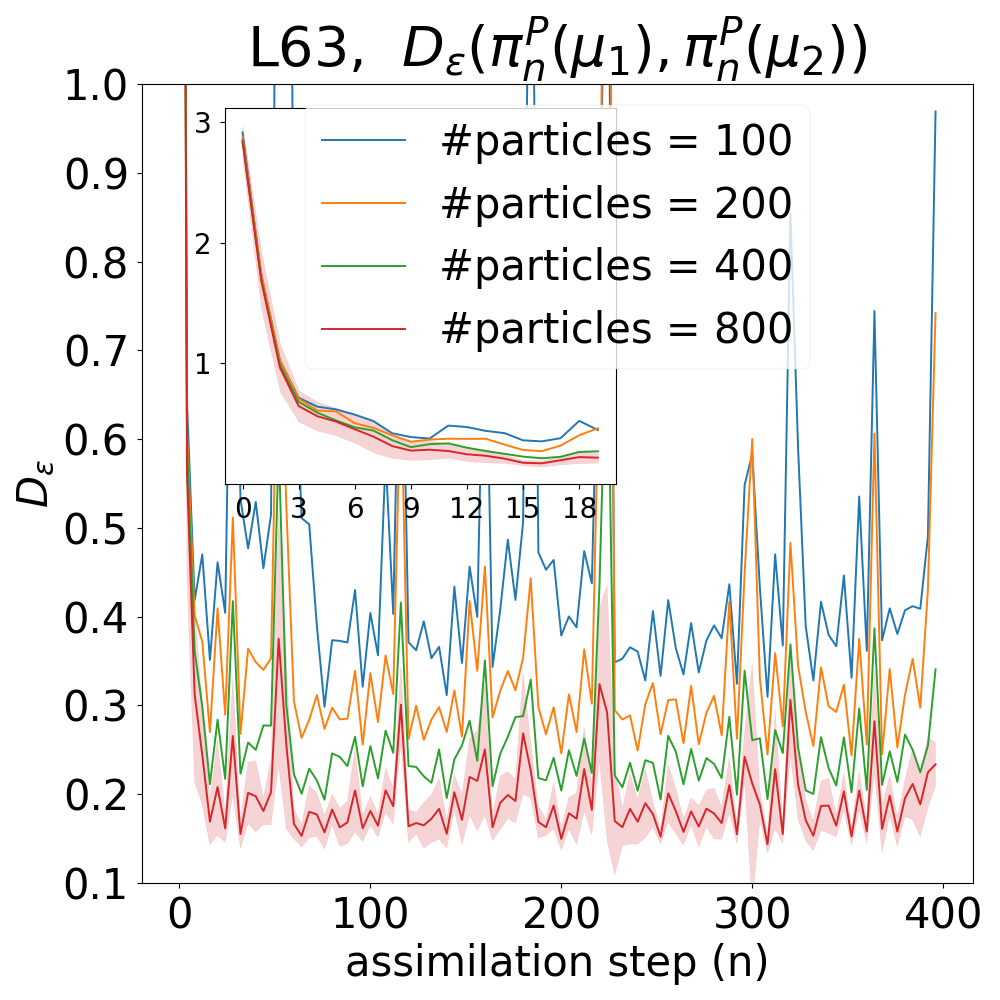
\includegraphics[width=0.2\textwidth]{stability/plots/figures-BPF-L63-0-dist_1_vs_2.png}} &
% {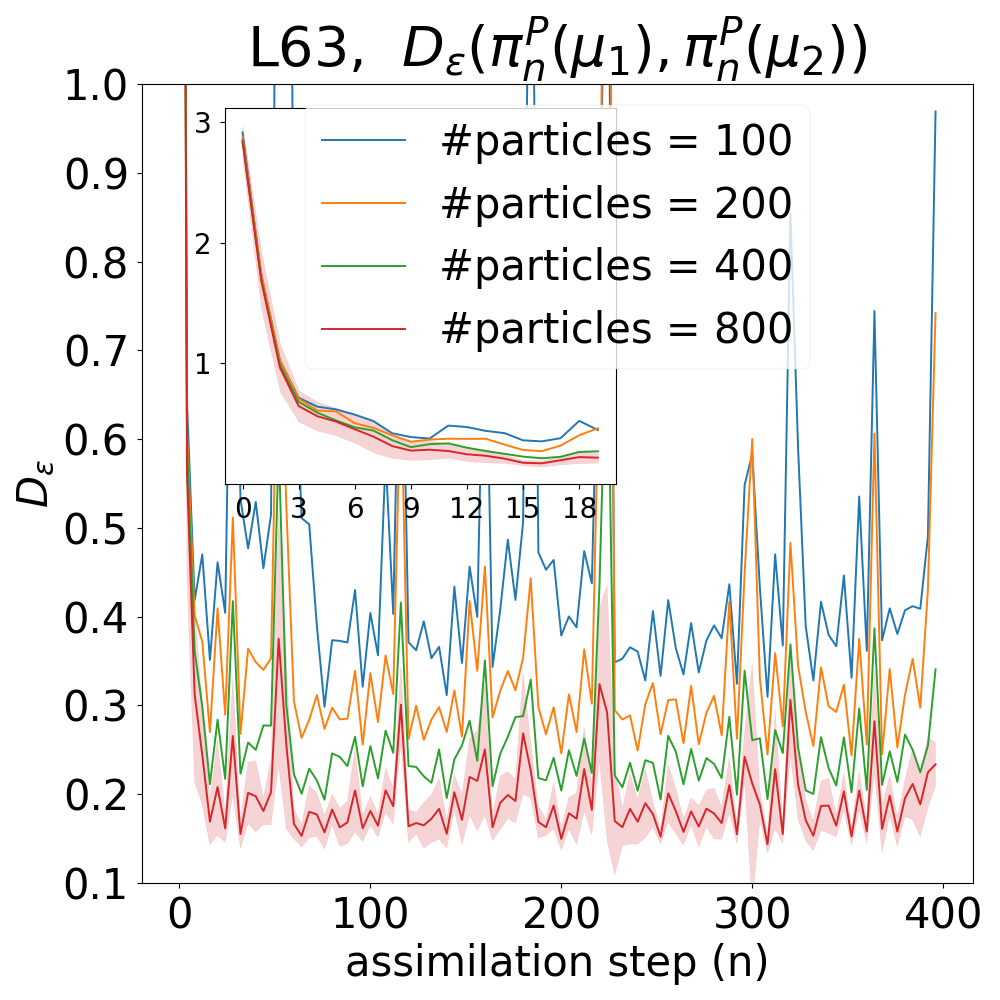
\includegraphics[width=0.2\textwidth]{stability/plots/figures-BPF-L63-0-dist_1_vs_2.png}} &
% {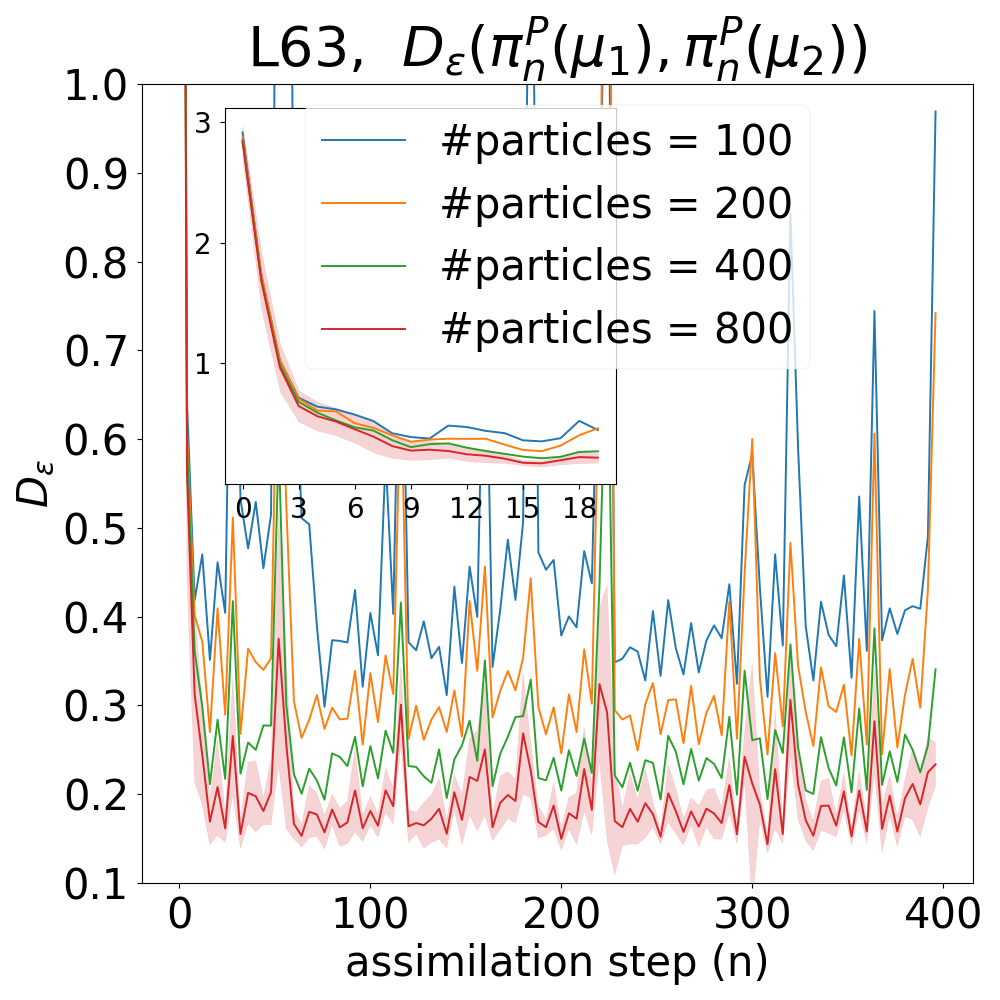
\includegraphics[width=0.2\textwidth]{stability/plots/figures-BPF-L63-0-dist_1_vs_2.png}} \\

% \end{tabular}
% \caption{Input Images}
% \end{figure*}




















